\documentclass[14pt]{article}

\usepackage[margin=1.5cm]{geometry}
\usepackage{enumerate}
\usepackage{amsmath,amssymb}
\usepackage{tikz}

\DeclareMathOperator{\proj}{proj}

\begin{document}

\begin{center}
Proficiency Exam 5 - Eigenvalues and Eigenvectors
\end{center}

You will have 30 minutes to complete the exam.  You may use a calculator, but you must show all steps done to get full credit for completing the problem.  This means that if you use your calculator for anything other than arithmetic, you must indicate on your test paper what you did on the calculator.

\begin{enumerate}

\item Consider the triangle with vertices (0,0), (2,5), and (6,2), depicted below.  What is the area of the triangle that results after applying the linear transformation
\[
T(\mathbf{x}) = \left[\begin{array}{cc} -2 & 1 \\ 3 & 5 \end{array}\right] \mathbf{x}?
\]

\begin{center}
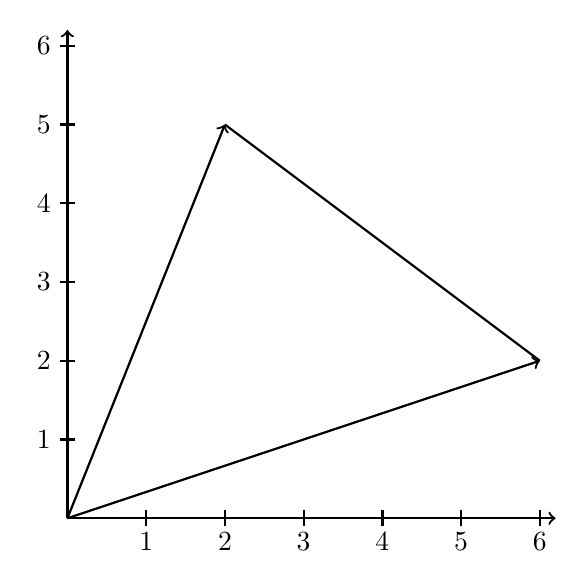
\begin{tikzpicture}
\draw[->,thick] (0,0) -- (2,5);
\draw[->,thick] (0,0) -- (6,2);
\draw[thick] (2,5) -- (6,2);

\draw[->,thick] (0,0) -- (0,6.2);
\draw[->,thick] (0,0) -- (6.2,0);
\draw[thick] (1,-0.1) -- (1,0.1);
\node at (1,-0.3) {1};
\draw[thick] (2,-0.1) -- (2,0.1);
\node at (2,-0.3) {2};
\draw[thick] (3,-0.1) -- (3,0.1);
\node at (3,-0.3) {3};
\draw[thick] (4,-0.1) -- (4,0.1);
\node at (4,-0.3) {4};
\draw[thick] (5,-0.1) -- (5,0.1);
\node at (5,-0.3) {5};
\draw[thick] (6,-0.1) -- (6,0.1);
\node at (6,-0.3) {6};
\draw[thick] (-0.1,1) -- (0.1,1);
\node at (-0.3,1) {1};
\draw[thick] (-0.1,2) -- (0.1,2);
\node at (-0.3,2) {2};
\draw[thick] (-0.1,3) -- (0.1,3);
\node at (-0.3,3) {3};
\draw[thick] (-0.1,4) -- (0.1,4);
\node at (-0.3,4) {4};
\draw[thick] (-0.1,5) -- (0.1,5);
\node at (-0.3,5) {5};
\draw[thick] (-0.1,6) -- (0.1,6);
\node at (-0.3,6) {6};
\end{tikzpicture}
\end{center}

\item The matrix $ A $ given below has an eigenvalue of $ -1 $.  Find a basis for the eigenspace (the subspace of all eigenvectors) for the eigenvalue of $ -1 $.
\[
A = \left[\begin{array}{ccc} 19 & 36 & -12 \\ -15 & -28 & 9 \\ -20 & -36 & 11 \end{array}\right]
\]

%\item Let $ A $ be a 2$\times$2 matrix with eigenvalues $ \lambda_1 = 1 $ and $ \lambda_2 = -2 $ with corresponding eigenvectors $ \mathbf{v_1} = \left[\begin{array}{c} 1 \\ 1 \end{array}\right] $ and $ \mathbf{v_2} = \left[\begin{array}{c} -1 \\ 1 \end{array}\right] $.  Find the matrix $ A $.

\item (TRUE or FALSE) Consider the statement and decide if it is true or false.  If true, provide reasoning.  If false, provide a counterexample.
\begin{center}
`` Suppose the matrix $ B $ is obtained from the matrix $ A $ by the row operation $ R_1 \rightarrow \alpha R_1 $.  Then $ \det(B) = \alpha\det(A) $.  "
\end{center}

\item Find the general solution to the following system of LODEs.
\begin{align*}
\frac{dx}{dt} &= 2x(t) - 1y(t) \\
\frac{dy}{dt} &= x(t) + 5y(t)
\end{align*}




























\end{enumerate}

\end{document}